\documentclass{IEEEtran}

\usepackage{amsmath}
\usepackage{listings}
\lstset{
    basicstyle=\small\ttfamily,
    breaklines=true
}
\usepackage{graphicx}
\graphicspath{ {./images/} }

\title{Readings about DP and Recursion}
\author{Diego Linares - kiwiAipom}

\begin{document}
    \maketitle

    \section{Everything about Dynamic Programming}

    \section{Some general approach for solving recursive problems}
        \textbf{Step One:} Think about any input for which you know what your function should return.\\
        Now suppose you have a task, related to a similar one. Keep calling that function to solve it: \textit{I'll solve the problem if you give me this subproblem first}. Which is done by a call to the same function.\\
        \textbf{Example:} With factorial, you only know that $0!=1$ and $n!=n(n-1)!$. So the function that gives me factorial of $n$ just needs the results of one that returns $(n-1)!$. This will keep going as long as we don't know whaat value to return.
        \begin{lstlisting}
factorial(n):
    if n = 0:
        return 1 // I know this, so I don't want my function to go any further
    else:
        return n*factorial(n-1) // just reuse the function
        \end{lstlisting}
        \textbf{Step Two:} They can do the same as loops, a simple \texttt{for} can be implemented as:
        \begin{lstlisting}
for(i, n):
    if i = n:
        return // Terminates
    // Do whatever needed
    for(i+1, n) // Next iteration
        \end{lstlisting}
        And for backwards:
        \begin{lstlisting}
rof(i, n):
    if i = n:
        return // Terminates
    rof(i+1, n) // Next iteration    
    // Do whatever needed
        \end{lstlisting}
        Since the function calls itself again until reaching a limit value and then starts returning.\\
        \textbf{Example:} To print numbers backwards you may do this:
        \begin{lstlisting}
function(i, n):
    if i <= n:
        function(i+1, n)
        print(i)
        \end{lstlisting}
        Which for numbers from 1 to 5 would work like:\\
        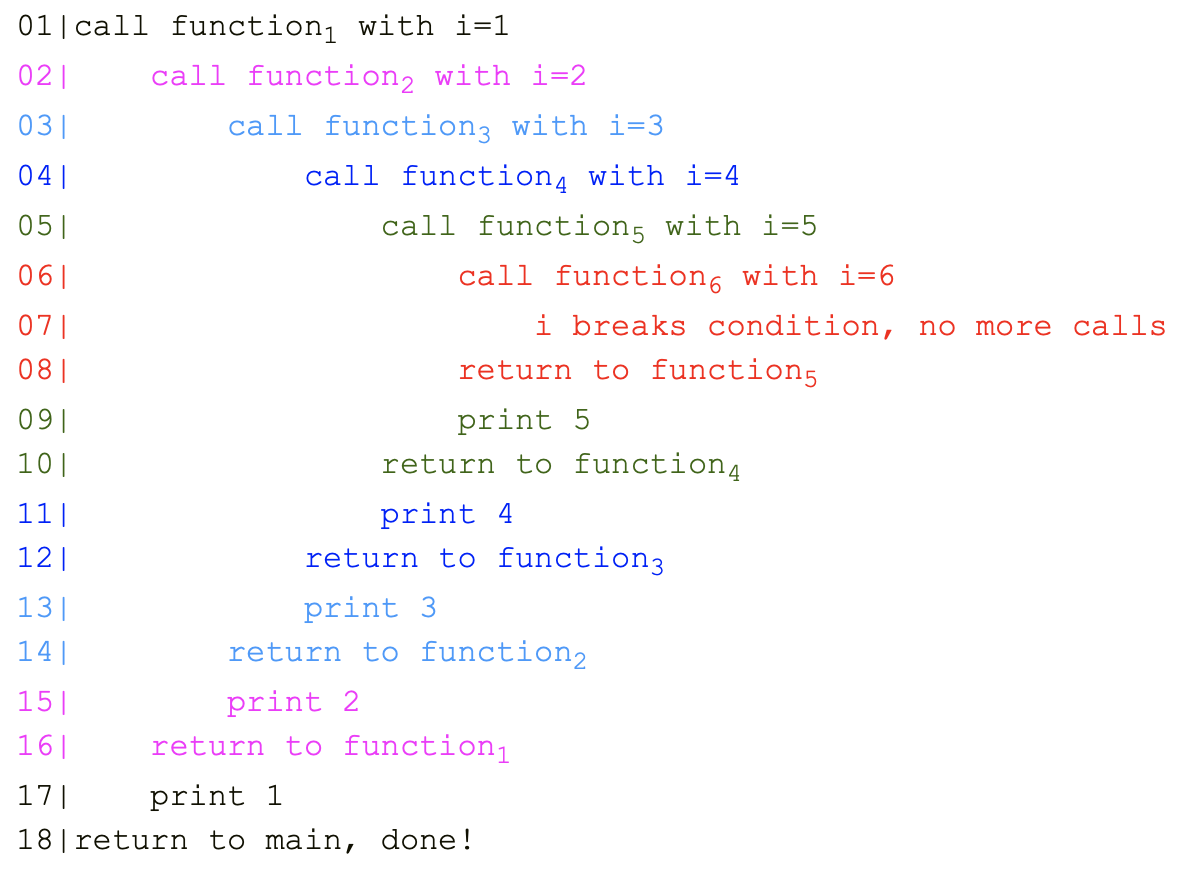
\includegraphics[width=0.4\textwidth]{rofExecution.png}\\
        \textbf{Step Three:} There's a stack call which looks like this:\\
        \begin{center}
            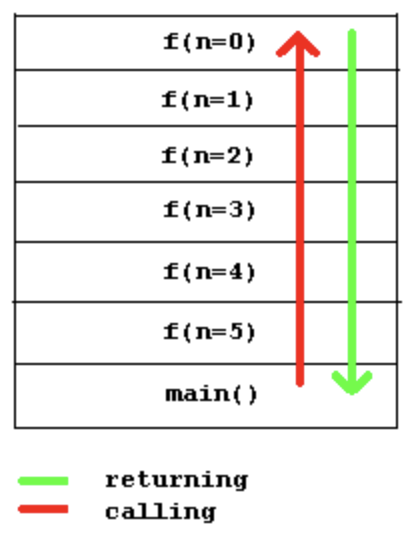
\includegraphics[width=0.15\textwidth]{stackCalls.png}
        \end{center}
        The memory of $f(3)$ for example, won't be freed until $f(2)$ is done. Serves the purpose of using an array, since the functions store variables and values.\\
        \textbf{Step Four:} Be careful, in CP they are generally avoided since most can be done iteratively, andd they may exceed time and memory. Since every function is alloted a space at the moment it is called, might run into RTE. Use only $O(\lg{n})$ and small $O(n)$ recursions. \\
        \textbf{Step Five:} When there are overlapping branches in the recursion tree we store computed values (DP).
    \section{Dynamic programming 2}
    \section{Matrix}
        \subsection{Cutting to the Chase}
            It can be slow if not done properly.\\
            \textbf{Example:} Obtain $x^n$ if multiplying is $O(1)$. Then $x^n=x*x*\ldots = O(N)$. We can reduce it like: $x^n=x^2*x^2*...$, and now the constant is now half. If we do $x^{\sqrt{n}}*x^{\sqrt{n}}*...$ and now the constant is $O(\sqrt{N})$\\
            So let's go faster. For even numbers $x^n=x^{\frac{n}{2}}*x^{\frac{n}{2}}$ and for odds $x^n = x^{\frac{n}{2}}*x^{\frac{n}{2}}*x$.\\
            Since the terms keep repeating themselves, we only need to calculate $x^{\frac{n}{2}}$ once and so on. This creates $O(\lg{n})$ complexity.\\
            Since matrices are an \textbf{associative mathematical structure}, this applies to it too.
        \subsection{Don't get stuck with struct}
            Matrix multiplication goes as such:\\
            $$
                \begin{bmatrix}
                    a_1&a_2\\
                    a_3&a_4
                \end{bmatrix}*
                \begin{bmatrix}
                    b_1&b_2\\
                    b_3&b_4
                \end{bmatrix}=
                \begin{bmatrix}
                    a_1*b_1+a_2*b_3&a_1*b_2+a_2*b_4\\
                    a_3*b_1+a_4*b_3&a_3*b_2+a_4*b_4
                \end{bmatrix}
            $$
            Basically, each row times each column of the other matrix. Now we can define a struct like:
            \begin{lstlisting}
struct Matrix
{
    int m[N][N];
    matrix()
    {
        memset(m,0,sizeof(m));
    }
    matrix operator * (matrix b)
    {
        matrix c = matrix();
        for(int i = 0; i < n; i++)
            for(int j = 0; j < n; j++)
                for(int k = 0; k < n; k++)
                    c.m[i][j] = c.m[i][j] + m[i][k] * b.m[k][j]
        return c;
    }
    matrix modPow(matrix m, int n)
    {
        if(n == 0)
            return unit;
        matrix half = modPow(m,n/2);
        matrix out = half * half;
        if(n % 2)
            out *= m;
        return out;
    }
}
            \end{lstlisting}
            The operator $*$ was defined so the matrix could be treated as a number. Unit refers to the unit matrix. 
        \subsection{N-th Fibonacci Term}
            Knowing how Fibonacci works, we can put it in the form of a matrix. Knowing that each term \textbf{is dependent on the previous two} we need a 2 row matrix. From the pair $(F_{n-2},F{n_1})$ we compute $(F_{n-1},F{n})$, like so:
            $$F_n=F_{n-1}*1+F_{n-2}*1$$
            $$F_{n-1}=F_{n-1}*1+F_{n-2}*0$$
            In the form of a matrix:
            $$
                \begin{bmatrix}
                    F_{n-2}&F_{n-1}\\
                    0&0
                \end{bmatrix}*
                \begin{bmatrix}
                    0&1\\
                    1&1
                \end{bmatrix}=
                \begin{bmatrix}
                    F_{n-1}&F_{n}\\
                    0&0
                \end{bmatrix}
            $$
            We can go one step back to see the pattern:
            $$
                \begin{bmatrix}
                    F_{n-3}&F_{n-2}\\
                    0&0
                \end{bmatrix}*
                \begin{bmatrix}
                    0&1\\
                    1&1
                \end{bmatrix}^2=
                \begin{bmatrix}
                    F_{n-2}&F_{n-1}\\
                    0&0
                \end{bmatrix}
            $$
            Finally
            $$
                \begin{bmatrix}
                    F_{1}&F_{2}\\
                    0&0
                \end{bmatrix}*
                \begin{bmatrix}
                    0&1\\
                    1&1
                \end{bmatrix}^{n-2}=
                \begin{bmatrix}
                    F_{n-1}&F_{n}\\
                    0&0
                \end{bmatrix}
            $$
            And we already know the power of a matrix is logarithmic.
        \subsection{Bits and Pieces}
            How many arrays of length $n$ with maximum $k$ consecutive 0 bits are.\\
            Supposing we can use DP for the problem. $D_{n.k}$ is the number of arrays of length $n$ which \textbf{end} in $k$ 0s.\\
            Considering a string can only be added a 0 or a 1. From $(n,k)$ we can go to $(n+1,k+1)$ (if we add 0) and $(n+1,0)$ (we add 1).\\
            So $D_{n,0} = \sum_{i=0}^k D_{n-1,i}$ (all the strings of length n which do not end in 0). And $D_{n,k}=D_{n-1,k-1}.$ So in recursive form:
            $$D_{n,0} = \sum_{i=0}^k D_{n-1,i}$$
            $$D_{n,1} = D_{n-1,0}$$
            $$D_{n,2} = D_{n-1,2}$$
            $$\cdots$$
            $$D_{n,k} = D_{n-1,k-1}$$
            And this can be explained through a matrix.
            $$
            \begin{bmatrix}
                D_{n-1,0}&D_{n-1,1}&\cdots&D_{n-1,k}\\
                0&0&\cdots&0\\
                \cdots&\cdots&&\cdots\\
                0&0&\cdots&0\\
                0&0&\cdots&0
            \end{bmatrix}*
            \begin{bmatrix}
                1&1&\cdots&0\\
                1&0&\cdots&0\\
                \cdots&\cdots&&\cdots\\
                1&0&\cdots&1\\
                1&0&\cdots&0
            \end{bmatrix}
            $$
            Yielding the result:
            $$
            \begin{bmatrix}
                D_{n,0}&D_{n,1}&\cdots&D_{n,k}\\
                0&0&\cdots&0\\
                \cdots&\cdots&&\cdots\\
                0&0&\cdots&0\\
                0&0&\cdots&0
            \end{bmatrix}
            $$
            The complexity is reduced from $O(n*k)$ to $O(\lg{n}*k^3)$, where $k^3$ is the complexity of multiplying the matrices. 
        \subsection{How big can it get?}
            This is a solution to the problem \textit{Chimney} from TopCoder. \textbf{Worth checking out}.
            \begin{lstlisting}
Layer 1      Layer 2
+-----+--+   +--+-----+
|  1  |  |   |  |  B  |
+--+--|2 |   | A+--+--+
|  |  |  |   |  |  |  |
| 4+--+--+   +--+--+C |
|  |  3  |   |  D  |  |
+--+-----+   +-----+--+
            \end{lstlisting}
            We need to find out the different orders in which bricks can be placed for $n$ layers, only restriction is that the 2 bricks that support the brick above are set before it.\\
            We can show it as a matrix here:
            \begin{lstlisting}
+-----+--+  +-----+--+  +-----+--+  +-----+--+ 
|xxxxx|  |  |     |  |  |xxxxx|  |  |     |xx|  
+--+--|  |  +--+--|  |  +--+--|  |  +--+--|xx|    
|  |  |  |  |xx|  |  |  |  |  |  |  |xx|  |xx|    
|  +--+--+  |xx+--+--+  |  +--+--+  |xx+--+--+  
|  |     |  |xx|xxxxx|  |  |xxxxx|  |xx|xxxxx|  
+--+-----+  +--+-----+  +--+-----+  +--+-----+   
    1            2           3           4

+-----+--+  +-----+--+  +-----+--+  +-----+--+
|     |  |  |     |xx|  |     |xx|  |     |xx|
+--+--|  |  +--+--|xx|  +--+--|xx|  +--+--|oo| 
+--+--|  |  +--+--|xx|  +--+--|xx|  +--+--|oo|
|xx|  |  |  |xx|  |oo|  |xx|  |oo|  |xx|  |oo|
|xx+--+--+  |xx+--+oo+  |xx+--+oo+  |xx+--+oo+
|=====xxx|  |xx|xxxoo|  |===== oo|  |===@@@@@|  
+--+-----+  +--+-----+  +--+-----+  +--+-----+ 
    5            6           7           8
            \end{lstlisting}
            Where $x$ are the bricks in $n$ layer, $o$ and $=$ in the $n+1$ and $@$ in the $n+2$. After we place 2 bricks next to the other we can put a brick in the layer above.\\
            Can be solved with matrix multiplication, $9*9$ matrix and multiplying it logarithmically. The base matrix being:
            \begin{lstlisting}
int mat[9][9] =  // constructing matrix column by column
    {{0,0,0,0,1,0,0,0,0},
    {4,0,0,0,0,0,1,0,0},
    {0,2,0,0,0,0,0,1,0},
    {0,1,0,0,0,0,0,0,0},
    {0,0,2,2,0,0,0,0,0},
    {0,0,1,0,0,0,0,0,1},
    {0,0,0,0,2,2,0,0,0},
    {0,0,0,0,0,0,1,0,0},
    {0,0,0,0,0,0,0,1,0}};
            \end{lstlisting}
        \subsection{Summing Up}
            Useful tool but not reccommended outside of contests.

\begin{thebibliography}{}
    \bibitem{mmi}
        \textit{Attacking Recursions},
        I, Me and Myself.
        From: https://zobayer.blogspot.com/2009/12/cse-102-attacking-recursion.html
    \bibitem{danalex}
        \textit{Matrix},
        DanAlex's blog,
        From: https://codeforces.com/blog/entry/21189
\end{thebibliography}

\end{document}